\documentclass[a4paper,UKenglish,cleveref]{lipics-v2019}

\usepackage[utf8]{inputenc}
\usepackage{amsmath}
\usepackage{amsfonts}
\usepackage{amssymb}
\usepackage{amsthm}
\usepackage{graphicx}
\usepackage{wrapfig}
\usepackage{makecell}
\usepackage{xspace}
\usepackage[usenames,dvipsnames]{xcolor}
\usepackage{caption}
\usepackage{wrapfig}
\usepackage{float}
\usepackage{booktabs}
%\usepackage[margin=0.7in,footskip=0.25in]{geometry}

%\newtheorem{definition}{Definition}
\newtheorem{condition}{Condition}
\newtheorem{conjecture}{Conjecture}
\newtheorem{observation}{Observation}
%\newtheorem{lemma}{Lemma}
%\newtheorem{theorem}{Theorem}

\newcommand{\mremark}[3]{\textcolor{blue}{\textsc{#1 #2:}} \textcolor{SeaGreen}{\textsf{#3}}}

\newcommand{\frank}[2][says]{\mremark{Frank}{#1}{#2}}
\newcommand{\maarten}[2][says]{\mremark{Maarten}{#1}{#2}}
\newcommand{\marc}[2][says]{\mremark{Marc}{#1}{#2}}
\newcommand{\jerome}[2][says]{\mremark{J\'er\^ome}{#1}{#2}}
\newcommand{\jordi}[2][says]{\mremark{Jordi}{#1}{#2}}
\newcommand{\ivor}[2][says]{\mremark{Ivor}{#1}{#2}}
\newcommand{\mees}[2][says]{\mremark{Mees}{#1}{#2}}
\newcommand{\todo}[2][DO]{\mremark{TO}{#1}{#2}}
\newcommand{\draw}{\todo{draw}}

\newcommand{\bigo}{\ensuremath{\mathcal O}}

\newcommand{\etal}{\textnormal{et al.}\xspace}
\newcommand{\spg}{\mathcal{S\!P}}
\newcommand{\ixi}{\mathcal{I}}
\newcommand{\pix}{\scalebox{0.6}{$\square$}}
\newcommand{\spix}{\boxplus}

\newcommand{\eps}{\varepsilon}
\newcommand{\R}{\mathbb{R}}

\graphicspath{Figures/}

\title{Mapping Multiple Regions to the Grid with Bounded Hausdorff Error}
\begin{document}
\maketitle

\section{Introduction}

\emph{Digital geometry} is concerned with the proper representation of geometric objects and their relationships using a grid of pixels. This greatly
simplifies both representation and many operations, but the downside is that common properties on geometric objects no longer hold. For example, it may be that two digitized lines intersect in multiple connected components. How to digitize a set of geometric objects so that such properties are guaranteed is one objective in digital geometry, referred to as \emph{consistency}. Another objective is the presentation of vector objects with bounded error, using subsets of pixels. Here we may assume the unit grid and measure error in one of multiple ways.

Early results in digital geometry were mostly concerned with consistency and arose in computer vision. For a survey, see Klette and Rosenfeld~\cite{klette2004digitalgeometry,klette2004digital}.
The interest from the algorithms community is more recent. Besides consistency, the Hausdorff error of digital representations is the topic of study.
Chun \etal~\cite{chun2009consistent} investigate the problem of digizing rays originating in the origin to digital rays such that certain properties are satisfied. They show that rays can be represented on the $n\times n$ grid in a consistent manner with Hausdorff error $O(\log n)$. This bound is tight in the worst case. By ignoring one of the consistency conditions, the error bound improves to $O(1)$.
Their research is extended by Christ \etal~\cite{christ2012consistent} to line segments (not necessarily starting in the origin), who obtain
the logarithmic error bound in this case as well.
A possible extension to curved rays was developed by Chun \etal~\cite{chun2019consistent}.
Other results with a digital geometry flavor within the algorithms community are those on snap rounding~\cite{de2007intersection,guibas,hershberger}, integer hulls~\cite{Althaus04,Harvey99}, and discrete schematization~\cite{loffler2017discretized}.

%The main motivation for using digital geometry is the fact representations are very simple and operations are simple, robust, and easily parallelizable. 
%it has also a large number of theoretical applications within computational geometry such as in snap rounding~\cite{de2007intersection}, integer precision geometry~\cite{harvey1999computing} and discrete schematization~\cite{loffler2017discretized}.

\begin{figure}[htb]
\centering
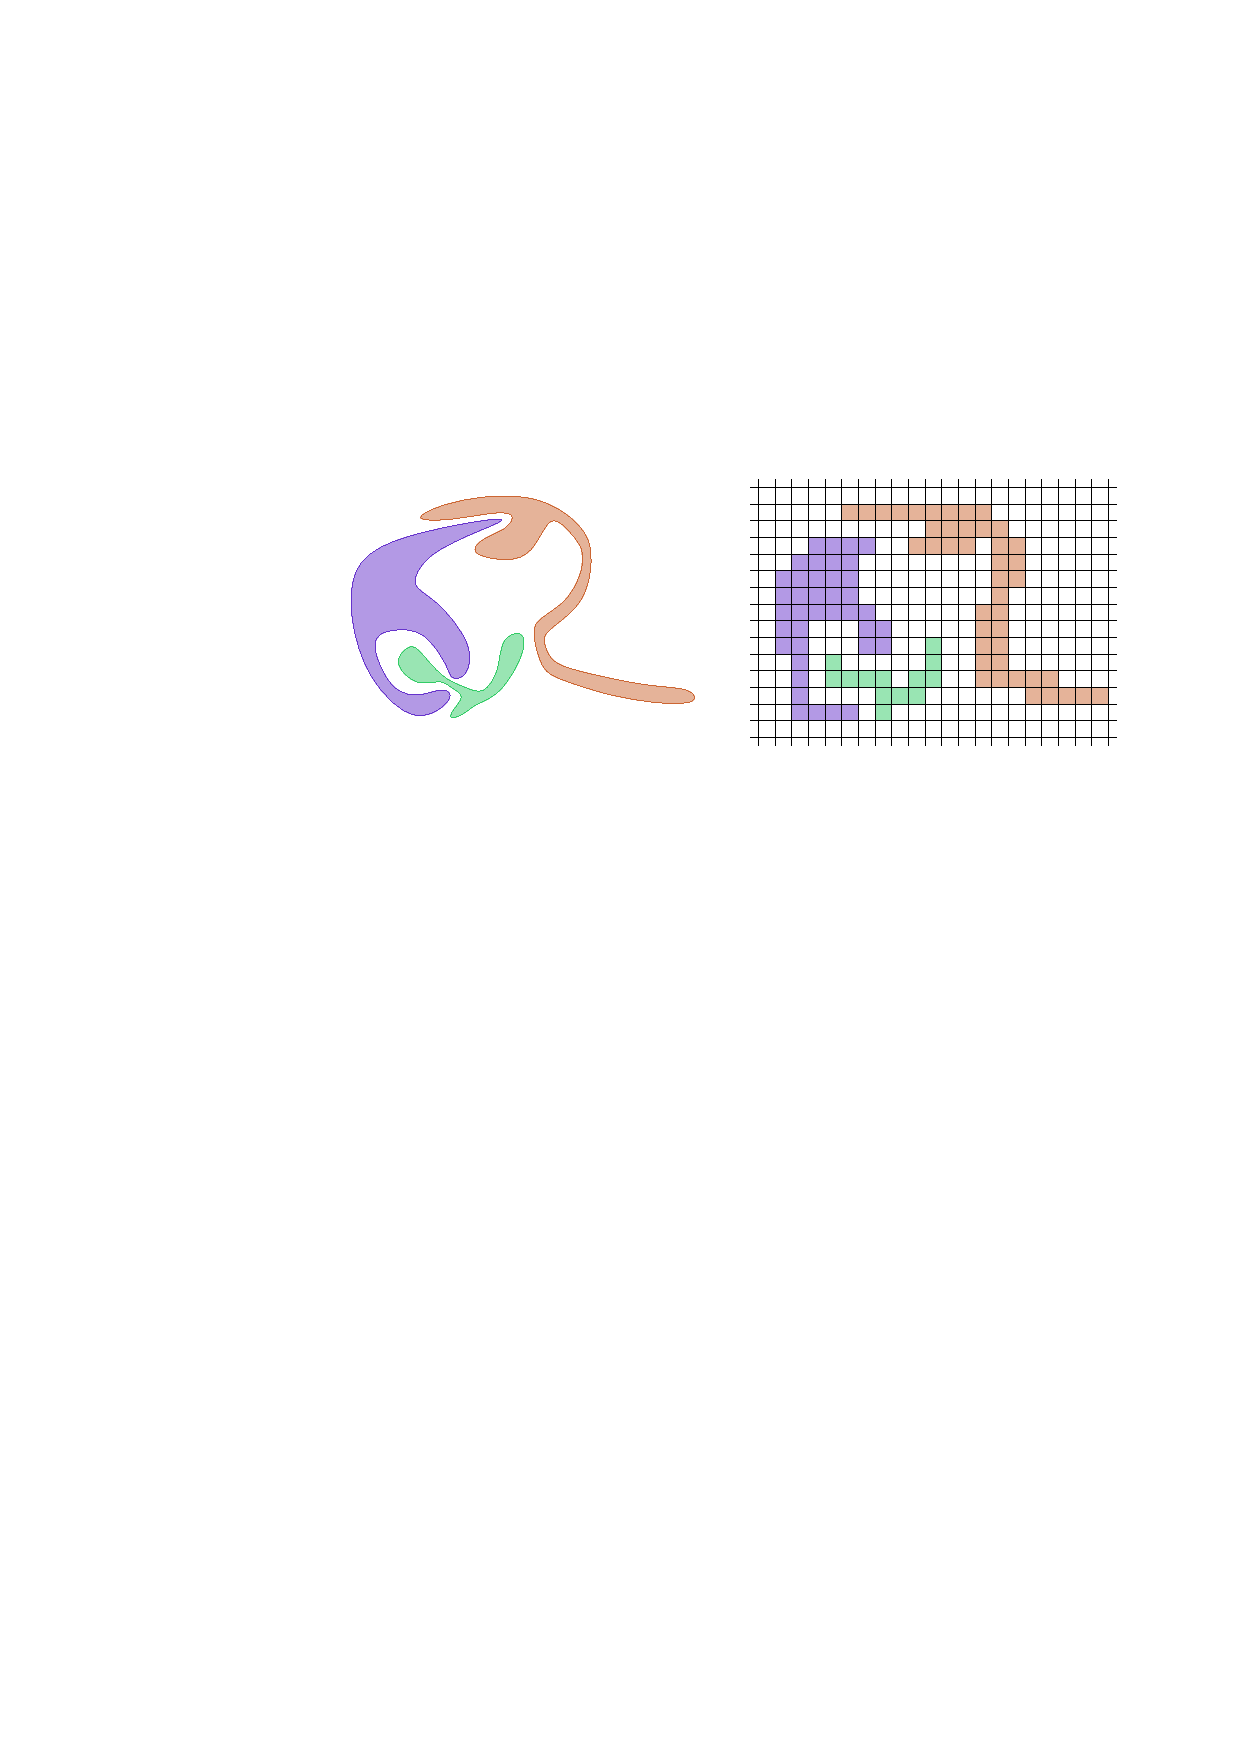
\includegraphics[]{Figures/introfig}
\caption{Three disjoint simply-connected regions and a representation by simply-connected sets of pixels.}
\label{fig:intro}
\end{figure}

In a recent paper, Bouts \etal~\cite{bouts2016mapping} showed that any simple polygon, no matter how detailed, can be represented by a simply-connected set of pixels such that the Hausdorff distance to and from the input is bounded by the constant $3\sqrt{2}/2$. They also prove that for the Fr\'echet distance between the boundaries, a constant error is not possible.
In this paper we extend the former result to multiple regions, see Figure~\ref{fig:intro} for an example. Depending on the size and shape characteristics of the regions, we obtain different bounds. We express our bounds in the number of regions to be represented by pixels. The precise results are given in Table~\ref{table:results}.


In this paper we consider a set $\mathcal{R}$ of $m$ simply connected regions and we wish to assign to each $R \in \mathcal{R}$ a simply connected set of pixels which represents $R$.
We investigate various restrictions on the set of regions $\mathcal{R}$ and we show that stricter restrictions allow for pixel representations with a smaller symmetric Hausdorff distance.



\begin{table}[H]
\begin{tabular}{lcc}
\toprule
Type of regions & Lower bound & Upper bound  \\ \midrule
point regions & $\Omega(\sqrt[]{m}) $ & $\bigo(\sqrt[]{m})$ \\
convex $\beta$-fat regions & $\Omega(\sqrt[]{m}) $ & $\bigo(\sqrt[]{m})$ \\
convex regions & $\Omega(m) $ & $\bigo(m)$ \\
two general regions &  $\Omega(1)$ & $\bigo(1)$\\
three general regions &  \multicolumn{2}{c}{unbounded}\\
\bottomrule\\
%$\Omega(2^m)$ & $\bigo(2^m)$ \\ \hline
\end{tabular}
\caption{A table representing our results for various restrictions on $\mathcal{R}$.}
\label{table:results}
\end{table}

\subparagraph{Notation and definitions.}
We denote by $\Gamma$ the (infinite) unit grid, whose unit squares are referred to as \emph{pixels}. 
%By $G_k \subset \Gamma$ we denote a \emph{subgrid of size} $k$, that is, an axis-aligned square that contains exactly $k \times k$ pixels of $\Gamma$. 
The {\em (symmetrical) Hausdorff distance} between two sets $A, B \subset \R^2$ is defined as $H(A, B) = \max \{\max_{a \in A}(\min_{b \in B}(|ab|)), \max_{b \in B}(\min_{a \in A}(|ab|))\}$. 
%Observe that the Hausdorff distance between any two closed sets is equal to the Hausdorff distance between their boundaries.\jordi{This is not true, the previous paper only proved this for the polygons that were being pixelised}
  
Consider a set of $m$ disjoint simply-connected regions $\mathcal{R} = \{R_1, R_2, \ldots R_m \}$ in the plane.
%that are contained in $G_k$ for some value of $k$. 
In this paper, we wish to assign to each region $R_i \in \mathcal{R}$ a simply-connected subset of the pixels $P_i \subset \Gamma$, such that the result is a set of $m$ disjoint simply-connected regions.
Two such \emph{grid polygons} are disjoint if they do not meet in any edge or vertex of the grid. A pixel polygon is connected if its pixels are connected by edge adjacency. A grid polygon is simply-connected if it is connected and its complement is also connected by edge adjacency. 
Hence, we do not allow vertex adjacency at all as it is ambiguous. In this paper a grid polygon is by default simply-connected.
We call the set $P_1, P_2, \ldots, P_m$ of such grid polygons a \emph{valid assignment}. An example is given in Figure~\ref{fig:intro}.

We are interested in finding for any set of regions $\mathcal{R}$ a valid assignment where for each region $R_i \in \mathcal{R}$, its corresponding grid polygon $P_i$ has a (symmetrical) Hausdorff distance to $R_i$ of at most $h$.
\jerome{and also the boundary?!}
In general, $h$ will be a function of $m$. We study this problem under several restrictions on $\mathcal{R}$: (1) the set $\mathcal{R}$ is a set of points, (2) the set $\mathcal{R}$ is a set of \emph{fat} convex regions, (3) the set $\mathcal{R}$ is a set of convex regions and (4) the set $\mathcal{R}$ is a set of arbitrary simply-connected regions.
For each class of restrictions, we derive a different bound on $h$. First we show that there is a set of regions in that class for which any valid assignment contains at least one region $R_i$ with a pixel polygon $P_i$ where $H(R_i, P_i) = \Omega(h)$. Second we show that for any set of regions in that class, we can find a valid assignment such that for all regions $R_i \in \mathcal{R}$ with corresponding grid polygon $P_i$, we have $H(R_i, P_i) = O(h)$. Hence, our bounds are asymptotically tight.

We may interpret any solution to our problem as a {\em coloring} of $\Gamma$ in the following way:
each pixel $\pix\in\Gamma$ can only be assigned one color. The set of colors is $C = \{c_1,\dots c_m\}\cup\{b\}$, where $c_i$ is the color of the input region $R_i$ and $b$ is the background color.
Formally the coloring is then a map $f:\Gamma\to C$. For each region $R_i$, its grid polygon $P_i$ is the union of all pixels in its color. A valid assignment yields a coloring where each color is simply-connected, and the background color $b$ is connected and has $m$ holes, see Figure~\ref{fig:intro}.

Our upper bound constructions follow a similar scheme. Let $\Gamma_k$ be a coarsening of the grid $\Gamma$ whose cells have $k\times k$ pixels. These cells are also called \emph{superpixels}. We will determine for each region from $\mathcal{R}$ which superpixels it contains and which ones it properly intersects.
If a region $R_i$ contains a superpixel, then all pixels of $\Gamma$ in that superpixel will be part of~$P_i$. If $R_i$ properly intersects a superpixel, we ensure that at least one but not all pixels in that superpixel will be part of~$P_i$. A superpixel not intersecting $R_i$ will have no pixels in~$P_i$.
The challenge that remains is finding a scheme by which each grid polygon becomes simply-connected. Assuming we succeed, then it is relatively straightforward to see that $H(R_i,P_i) \le k\sqrt{2}$. This bound also holds for the symmetric Hausdorff distance between the boundaries of $R_i$ and~$P_i$.

The remainder of this paper is organized as follows. We start with the easy case of point regions in Section~\ref{sec:points} and show an asymptotically tight bound of $\Theta(\sqrt{m})$. Then we proceed with $\beta$-fat convex regions and show the same bound in
Section~\ref{sec:fat}, assuming $\beta$ is a constant. When the regions are convex but not necessarily fat, we prove a bound of $\Theta(m)$ in Section~\ref{sec:convex}. Finally, we consider general regions and extend the $O(1)$ Hausdorff bound of Bouts \etal~\cite{bouts2016mapping} from one to two regions
in Section~\ref{sec:general}. In that section we also show that the bound does not extend to more regions: the Hausdorff distance may be unbounded already for three general regions.




%For all cases of $\mathcal{R}$, we follow the same approach to construct the desired result: suppose we are given $\mathcal{R}$ in a grid $G_{c \cdot k}$ for specified constants $c$ and $k$ and that we want to find a valid assignment of pixels $P_1 \ldots P_m$ where for each region $R_i$, $H(R_i, P_i) \le \sqrt{2}c$. Then we partition $G_{c \dot k}$ into $k^2$ \emph{superpixels} $\mathcal{S}$ of \emph{size} $c$ (each superpixel $S \in \mathcal{S}$ is an axis-aligned square containing $c^2$ pixels). Let $R_i$ be a region that intersects a set $\mathcal{S}$ of superpixels. Let $P_i$ be any assignment of pixels that only places pixels in $\mathcal{S}$, and that places at least one pixel in each superpixel in $\mathcal{S}$. Then $H(R_i, P_i) \le \sqrt{2}c$.

\section{Input regions are points.}
\label{sec:points}
In this section, we assume that $\mathcal{R}$ is a set of points. We will construct a map that assigns points to pixels such that the symmetric Hausdorff distance between each point and its corresponding pixel is bounded. 
%Surprisingly, we can show that even if the set $\mathcal{R}$ consists of points (which are the simplest form of regions) then it is still not always possible to find a valid assignment whose symmetric Hausdorff distance to $\mathcal{R}$ is bound by a constant: 
For a lower bound, consider a set of $m$ points $\mathcal{R}$ that all lie within a single pixel. 
If we want to assign each point to a unique pixel, we clearly need to use $m$ different pixels. Any set of $m$ pixels has diameter $\Omega(\sqrt{m})$, so at least
one of the point regions will be mapped to a pixel at distance $\Omega(\sqrt{m})$. Requiring disjointness of the pixels increases the lower bound, but only by a constant factor.

We now present a scheme that maps any set of $m$ points $\mathcal{R}$ to a set of pixels, such that the symmetric Hausdorff distance between any point and its pixel is at most $\mathcal{O}(\sqrt{m})$. Let $\Gamma_k$ be a coarsening of $\Gamma$ with $k=2\lceil \sqrt{k}\rceil$. Associate each region in 
$\mathcal{R}$ with the superpixel that contains it. Each superpixel has the space to accommodate $m$ disjoint pixels without using the bottom row and right column by using exactly the odd numbered rows and columns. We make any assignment of the points to these pixels in the same superpixel. The result is easily seen to have Hausdorff distance $O(\sqrt{m})$.

%The subgrid $G_k$ contains at most $(\lfloor \frac{k}{2\sqrt{m}} \rfloor)^2$ superpixels of size $2\sqrt{m}$. We overlay $G_k$ with a slightly larger grid $G'$ that contains $(\lceil \frac{k}{2\sqrt{m}} \rceil)^2$ superpixels of size $2\sqrt{m}$ each. For every point $R_i$ we identify which superpixel $S \subset G'$ contains $R_i$. Consider the lexicographical order of the pixels in $S$. We assign $R_i$ to the $2i$'th pixel in this lexicographical order. Since the indexing on $\mathcal{R}$ is fixed, each point gets assigned to a unique pixel. Moreover, each point gets assigned to a superpixel of size $2\sqrt{m}$ that contains the point. It follows that we have found an assignment of mutually disjoint pixels that each have a distance of at most $2\sqrt{m}$ to their corresponding point. Thus we conclude:

\begin{theorem}
If $\mathcal{R}$ is a set of points, it is possible to find a valid assignment such that for each region $R_i \in \mathcal{R}$ with a corresponding region $P_i$, we have $H(R_i, P_i) = \Theta(\sqrt{m})$.
\end{theorem}

\section{Input regions are convex $\beta$-fat regions.}
\label{sec:fat}

A $\beta$-fat region $R$ is a connected region with an assigned center point $p \in R$, such that the incircle of $R$ with center $p$ and the excircle of $R$ with center $p$ have a radius which differs by at most a factor $\beta$. Observe that the only regions which are $1$-fat are disks and points. In this section we consider the class $\mathcal{R}$ of convex $\beta$-fat regions for constant $\beta$. Points are $\beta$-fat regions for \emph{any} $\beta$, so from Section~\ref{sec:points} it follows that for any $m$, there exists a set of $m$ regions for which the symmetric Hausdorff distance between $\mathcal{R}$ and any valid assignment is $\Omega(\sqrt{m})$.

We continue to present an algorithm that maps any set of $\beta$-fat convex regions to a valid assignment, such that the symmetric Hausdorff distance between any region $R_i$ and its assigned region $P_i$ is at most $\mathcal{O}(\beta \sqrt{m})$. Let $\mathcal{R}$ be a set of $\beta$-fat regions in a subgrid $G_k$ for a constant $k$. Just as in Section~\ref{sec:points}, we overlay $G_k$ with a slightly larger grid that contains $(\lceil \frac{k}{2\sqrt{m}} \rceil)^2$ superpixels of size $2\sqrt{m}$. Observe that any $\beta$-fat region $R_i$ can intersect at most $8\beta$ superpixels without covering at least one superpixel. This leads to the following algorithm: for each region $R_i$, let $\mathcal{S}_i$ be the set of superpixels that are contained in $R_i$. If $\mathcal{S}_i$ is empty, then we arbitrarily select a superpixel $S$ that is intersected by $R_i$ and we assign $R_i$ to a unique pixel in $S$ according to the procedure in Section~\ref{sec:points}. This unique pixel has a distance of at most $16\beta \sqrt{m}$ to any other point on $R_i$ since else $R_i$ must intersect more than $8\beta$ superpixels which would make $\mathcal{S}_i$ non-empty. If $\mathcal{S}_i$ is not empty, we assign all pixels in each superpixel of $\mathcal{S}_i$ to $R_i$. Because $R_i$ is convex, the set $\mathcal{S}_i$ has to be connected. Moreover, each point of $R_i$ has a distance of at most $16\beta \sqrt{m}$ to the closest filled superpixel, for the same reasons as we presented above. Thus, we conclude the following:


\begin{theorem}
If $\mathcal{R}$ is a set of $\beta$-fat convex regions for a constant $\beta$, it is possible to find a valid assignment such that for each region $R_i \in \mathcal{R}$ with a corresponding region $P_i$, $H(R_i, P_i) = \Theta(\beta\sqrt{m})$.
\end{theorem}


\section{Input regions are convex regions.}\label{sec:convex}
Let the regions have as their only requirement that they are convex. In that case we can immediately show that the coloring has a lower-bound Hausdorff distance of $\Theta(m)$. The construction is shown in Figure \ref{fig:linesexample}.

\begin{figure}
\centering
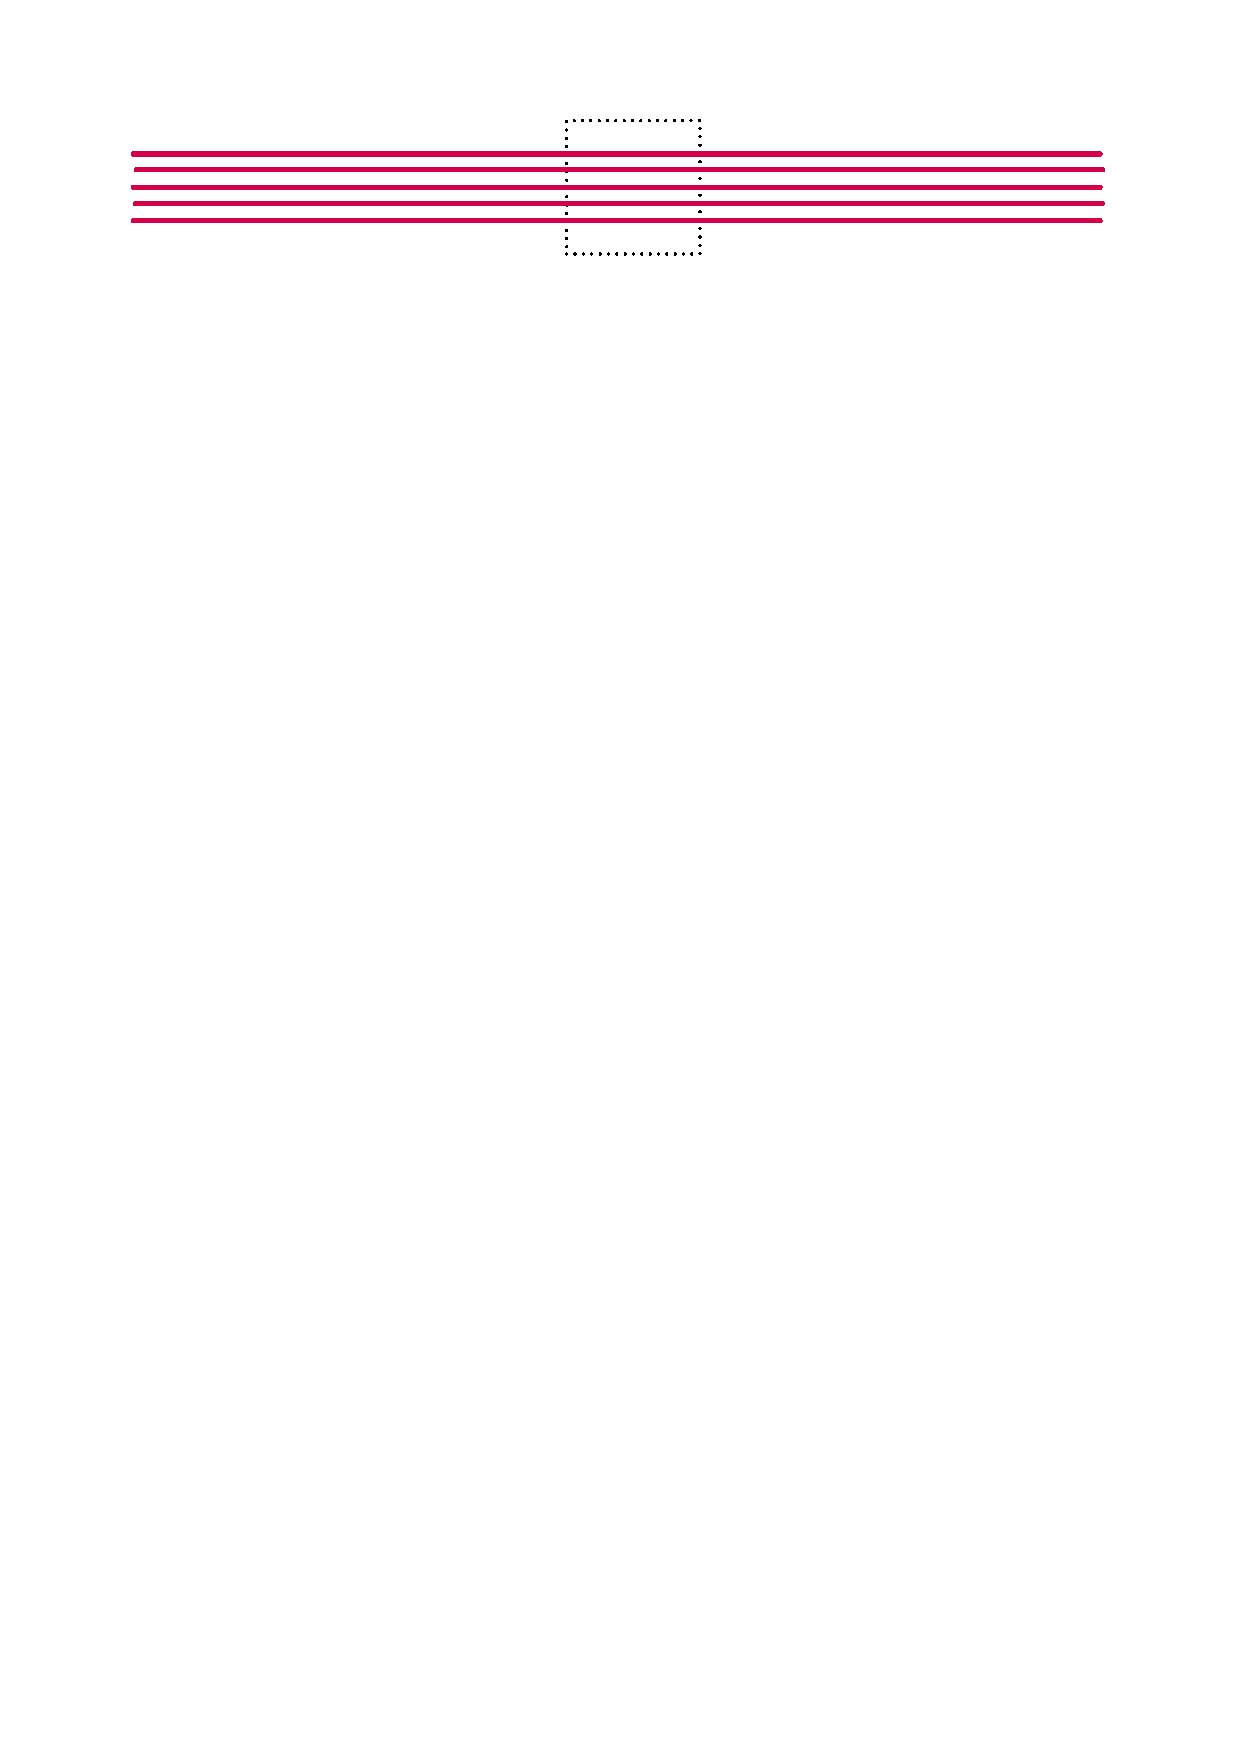
\includegraphics[scale=0.8]{Figures/linesexample.pdf}
\caption{The dotted square is a pixel. We can let $m$ vertical lines intersect the pixel. If their length is far greater than $m$, we can only project these regions to $m$ disjoint lines of pixels, which means that the outer lines must have a Hausdorff distance of $\Theta(m)$.}
\label{fig:linesexample}
\end{figure}

We will describe an algorithm that, given a set of convex regions \(\mathcal{R}\), gives a set of orthoconvex grid polygons \(\mathcal{P}\) such that \(\mathcal{R}\) and \(\mathcal{P}\) are \(\Theta(m)\)-similar.

\begin{observation}\label{obs:convex-ordering}
Let \(R_1,R_2 \in \mathcal{R}\) be two convex regions. A horizontal line that intersects both regions will have them appear in a certain left-to-right order. There cannot be another horizontal line where this order is reversed. A symmetrical property holds for vertical lines, where there is a top-to-bottom order.
\end{observation}

\cref{obs:convex-ordering} allows us to define two partial orders \(\preceq_x\) and \(\preceq_y\) on \(\mathcal{R}\): \(R_i \preceq_x R_j\) iff the leftmost point in \(R_i\) does not lie to the right of the leftmost point in \(R_j\), and \(R_i \preceq_y R_j\) iff the topmost point in \(R_i\) does not lie below the topmost point in \(R_j\). Now let \(X_\mathcal{R}\) and \(Y_\mathcal{R}\) be two indices on \(R\) that respect \(\preceq_x\) and \(\preceq_y\), respectively, and let \(k\Gamma\) be a superpixel grid with \(k = 2m\). Finally, for any superpixel \(\spix \in k\Gamma\), we denote by \(\spix[x, y]\) the pixel that is the \(2x\)th from the left and \(2y\)th from the top within \(\spix\).

Our algorithm works as follows:

\begin{enumerate}
	\item For each superpixel \(\spix\) that is intersected by a region \(R_i\), we color \(\spix[X_\mathcal{R}(R_i), Y_\mathcal{R}(R_i)]\) with \(c_i\).
	\item For any two pixels that are colored with \(c_i\) in adjacent superpixels, we color all pixels on the straight line segment between them with \(c_i\) as well.
	\item For any four superpixels that form a cycle in \(G\), if they each contain a pixel colored with \(c_i\) in Step 1, we color all pixels in the square between these pixels with \(c_i\) as well.
\end{enumerate}

\noindent
See \cref{fig:convexprojection} for an illustration.

\begin{figure}
\centering
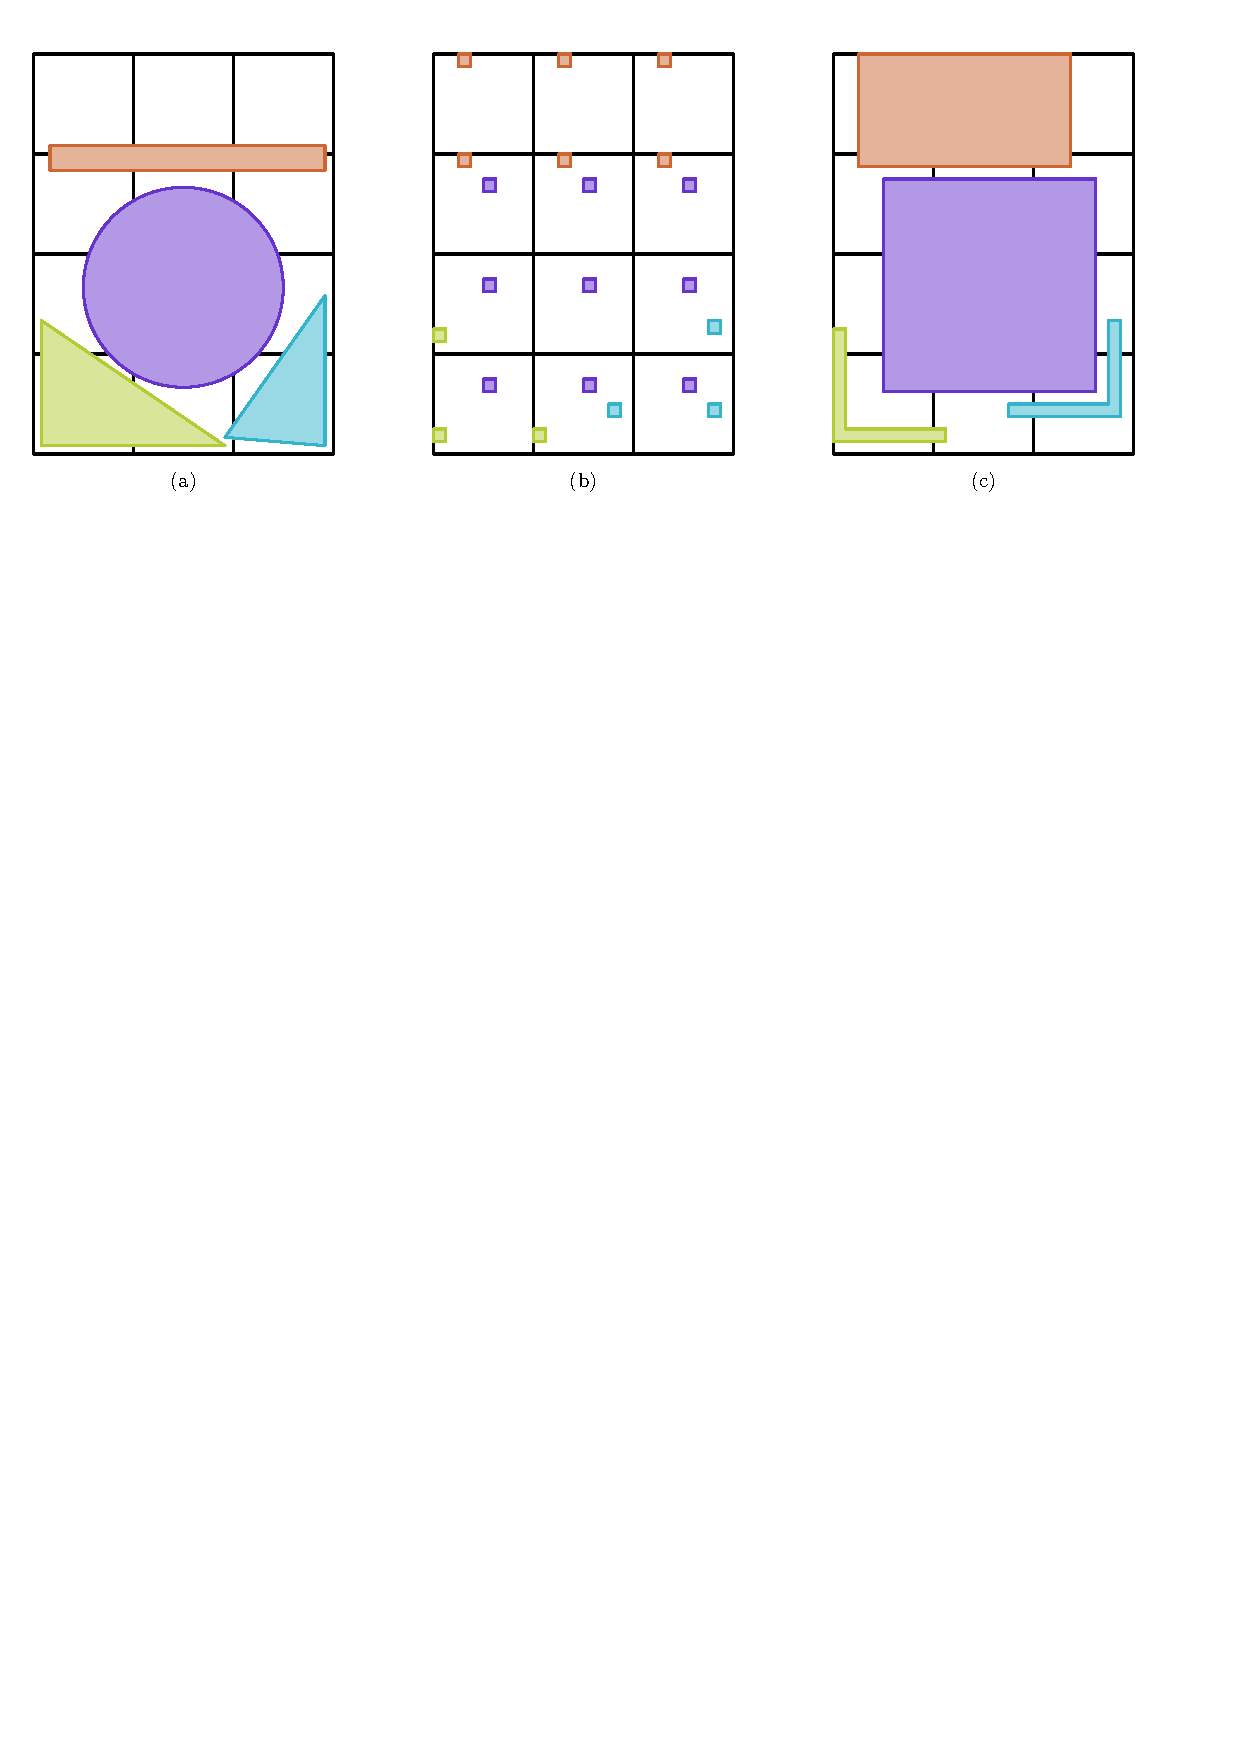
\includegraphics[width=\textwidth]{Figures/convexprojection.pdf}
\caption{The coloring algorithm for convex regions. (a) shows the input of four convex regions, overlaid onto a superpixel grid with \(k = 8\). (b) shows the pixels colored in Step 1 of the algorithm. (c) shows the final coloring obtained after Steps 2 and 3.}
\label{fig:convexprojection}
\end{figure}

Let \(f\) be the coloring obtained by the algorithm above.

\begin{lemma}\label{lem:convex-simply-connected}
	The polygons induced by \(f\) are simply connected.
\end{lemma}
\begin{proof}
	Consider a polygon \(P_i\) induced by \(f\). Its connectedness follows directly from the connectedness of the polygons in the input: \(R_i\) must intersect a connected set of superpixels, and our algorithm connects all of these together. It also cannot contain holes: the presence of a hole would imply that the set of superpixels intersected by \(R_i\) contains a hole, which is not possible due to \(R_i\) being simply connected and convex.
\end{proof}

\begin{figure}[tb]
\centering
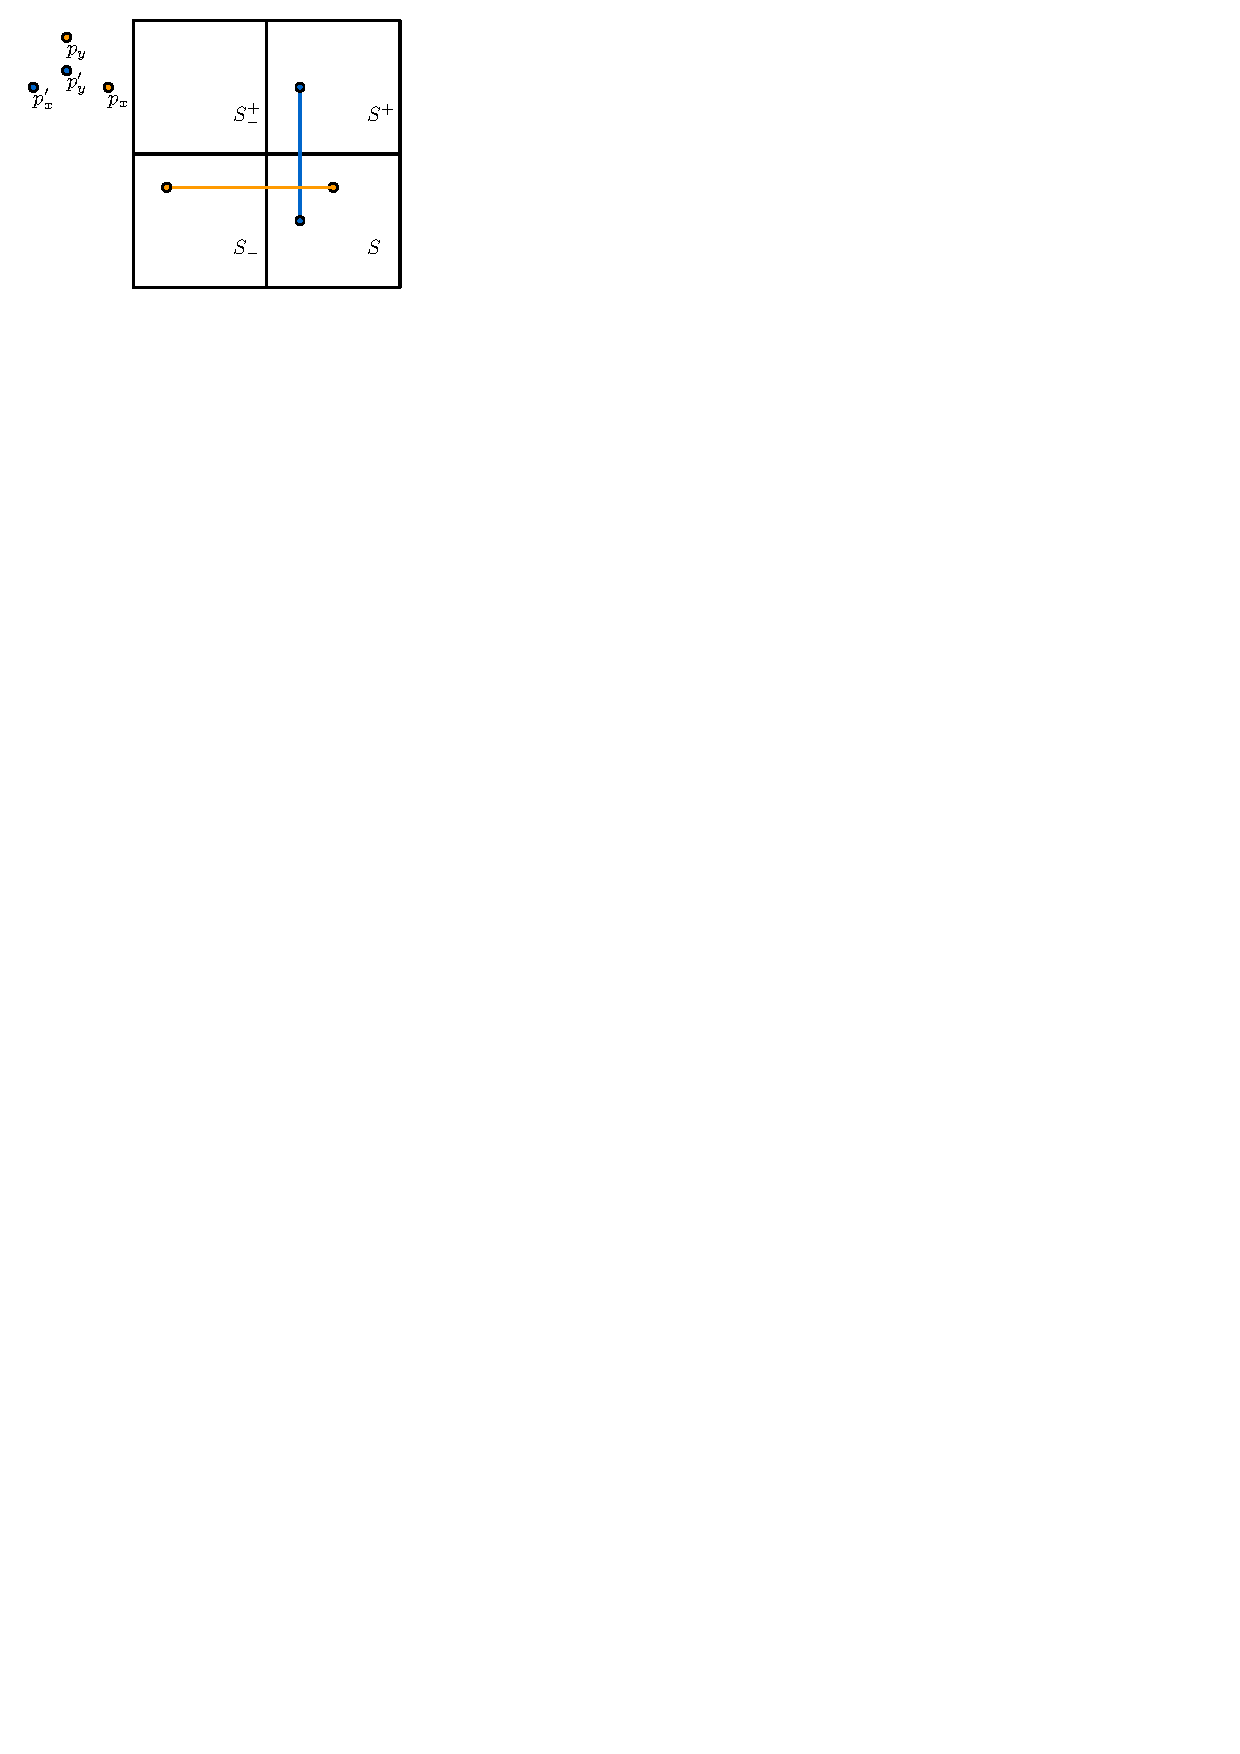
\includegraphics{intersection.pdf}
\caption{An assignment of pixels such that two assigned polygons (the blue and the orange) intersect whenever you connect the pixels. }
\label{fig:intersection}
\end{figure}

\begin{lemma}\label{lem:convex-separated}
	The polygons induced by \(f\) are separated by the background color.
\end{lemma}
\begin{proof}
	The coloring obtained in Step 1 is separated by construction; it remains to be shown that the pixels colored in Steps 2 and 3 are also separated.

	In Step 2, we only color horizontal and vertical sequences of pixels, and as each color has a unique row and column in each superpixel, it suffices to show that a horizontal sequence of color \(c_i\) never intersects a vertical sequence of color \(c_j\). Assume that two such sequences do intersect; there must be one superpixel \(S\) in which both colors are present. From \(S\), the horizontal sequence extends to the superpixel to the left or right, and the vertical sequence extends to the superpixel above or below. Assume w.l.o.g. one color appears in pixel \(S[x,y]\) and extends to the right, and that another color appears in pixel \(S[u,v]\) and extends downward (the other cases are symmetrical).

	As the sequences intersect, we have that \(x \leq u\) and \(v \leq y\). This implies that \(R_i \preceq_x R_j\) and \(R_j \preceq_y R_i\); note that either of these orders needs to be strict, otherwise \(R_i\) and \(R_j\) intersect. This means that either \(R_i\) contains a point strictly to the left of the leftmost point of \(R_j\), and \(R_j\) crosses from above \(R_i\) to below, or \(R_j\) contains a point strictly above the topmost point of \(R_i\), and \(R_i\) crosses from the left of \(R_j\) to the right. Both cases imply that \(R_i\) and \(R_j\) intersect, which contradicts our assumptions on the input. We conclude that no horizontal and vertical sequence can intersect, and that therefore Step 2 maintains the separation of colors.

	For Step 3 to cause an intersection, we would need to have a pixel \(S[x,y]\) with color \(c_i\) inside a region being filled with color \(c_j\). Let \(S[u,v]\) be the pixel in \(S\) with color \(c_j\); assume w.l.o.g. that \(x > u\) and \(y > v\) (again, the other cases are symmetrical). For an intersection to occur, we must be filling a square with color \(c_j\) to the bottom right from \(S[u,v]\). By the same argument as used for Step 2, this means that \(R_j\) crosses from the top or left of \(R_i\) to the right or bottom, which is only possible if \(R_i\) and \(R_j\) intersect.

	We conclude that none of the steps in the algorithm can violate the separation of the colors in \(f\), which implies that the induced polygons are separated by the background color.
\end{proof}

\begin{theorem}
	The polygons \(\mathcal{P}\) induced by \(f\) are \(\Theta(m)\)-similar to \(\mathcal{R}\).
\end{theorem}
\begin{proof}
	By \cref{lem:convex-simply-connected,lem:convex-separated}, \(f\) is a valid coloring. By construction, \(P_i\) intersects any superpixel that \(R_i\) does. Furthermore, any \(R_i\) that contains a superpixel \(S\) necessarily intersects all surrounding superpixels. As such, \(S\) will be completely filled with color \(c_i\) in Step 3 of the algorithm, implying that \(P_i\) also contains \(S\). These two facts combined imply that \(f\) respects the superpixel grid, which lets us apply \cref{lem:respect_means_bound} to obtain the bound.
\end{proof}

\section{Input regions are general regions.}
\label{sec:general}

When the input regions are arbitrary, we see a sharp contrast between one or two regions, where constant Hausdorff distance can be realized, and three or more regions, where the Hausdorff distance may be unbounded.
The fact that one region can be represented as a grid polygon with constant Hausdorff distance was shown before by Bouts \etal~\cite{bouts2016mapping}. In Section~\ref{subsec:two} we show that the same result holds for two regions. In Section~\ref{subsec:three}
we show that for three regions, no bounded Hausdorff distance bound exists that applies to all input.

\subsection{Two Regions}
\label{subsec:two}

Our result for two arbitrary regions is based on
a result on the Painter's Problem in \cite{goethem2017painter}.
A Painter's Problem instance takes a grid, and for each cell, the color white, blue, red, or purple. White indicates the absence of red and blue while purple indicates the presence of both red and blue. So in
essence, there are only two colors.
The question is whether two disjoint simply-connected regions for red and blue exist that is consistent with all specifications of the
cells, or, in their terminology, ``admits a painting''. Since red cells can simply be colored red and blue cells blue, the problem boils down to recoloring the purple cells with red and blue pieces. The red and blue pieces in a cell provide a panel, and all panels together make up a painting. They prove:

\begin{lemma} {\bf (Lemma 8 in \cite{goethem2017painter})}
\label{lem:painting}
If a 2-colored grid admits a painting, then it admits a painting where each panel has at most 3 intervals of alternating red and blue along each side.
\end{lemma}

The intervals on the sides make sure that the overall red and blue parts are connected across the whole painting.

They proceed to show that several configurations can be reduced to others, or simplified. For example, intervals that are not connected to other intervals on that panel can be removed (unless they were the last one of their color), and two adjacent sides with three intervals can be assumed to have the same colored interval in the corner where these sides meet.

\begin{figure}[tb]
\centering
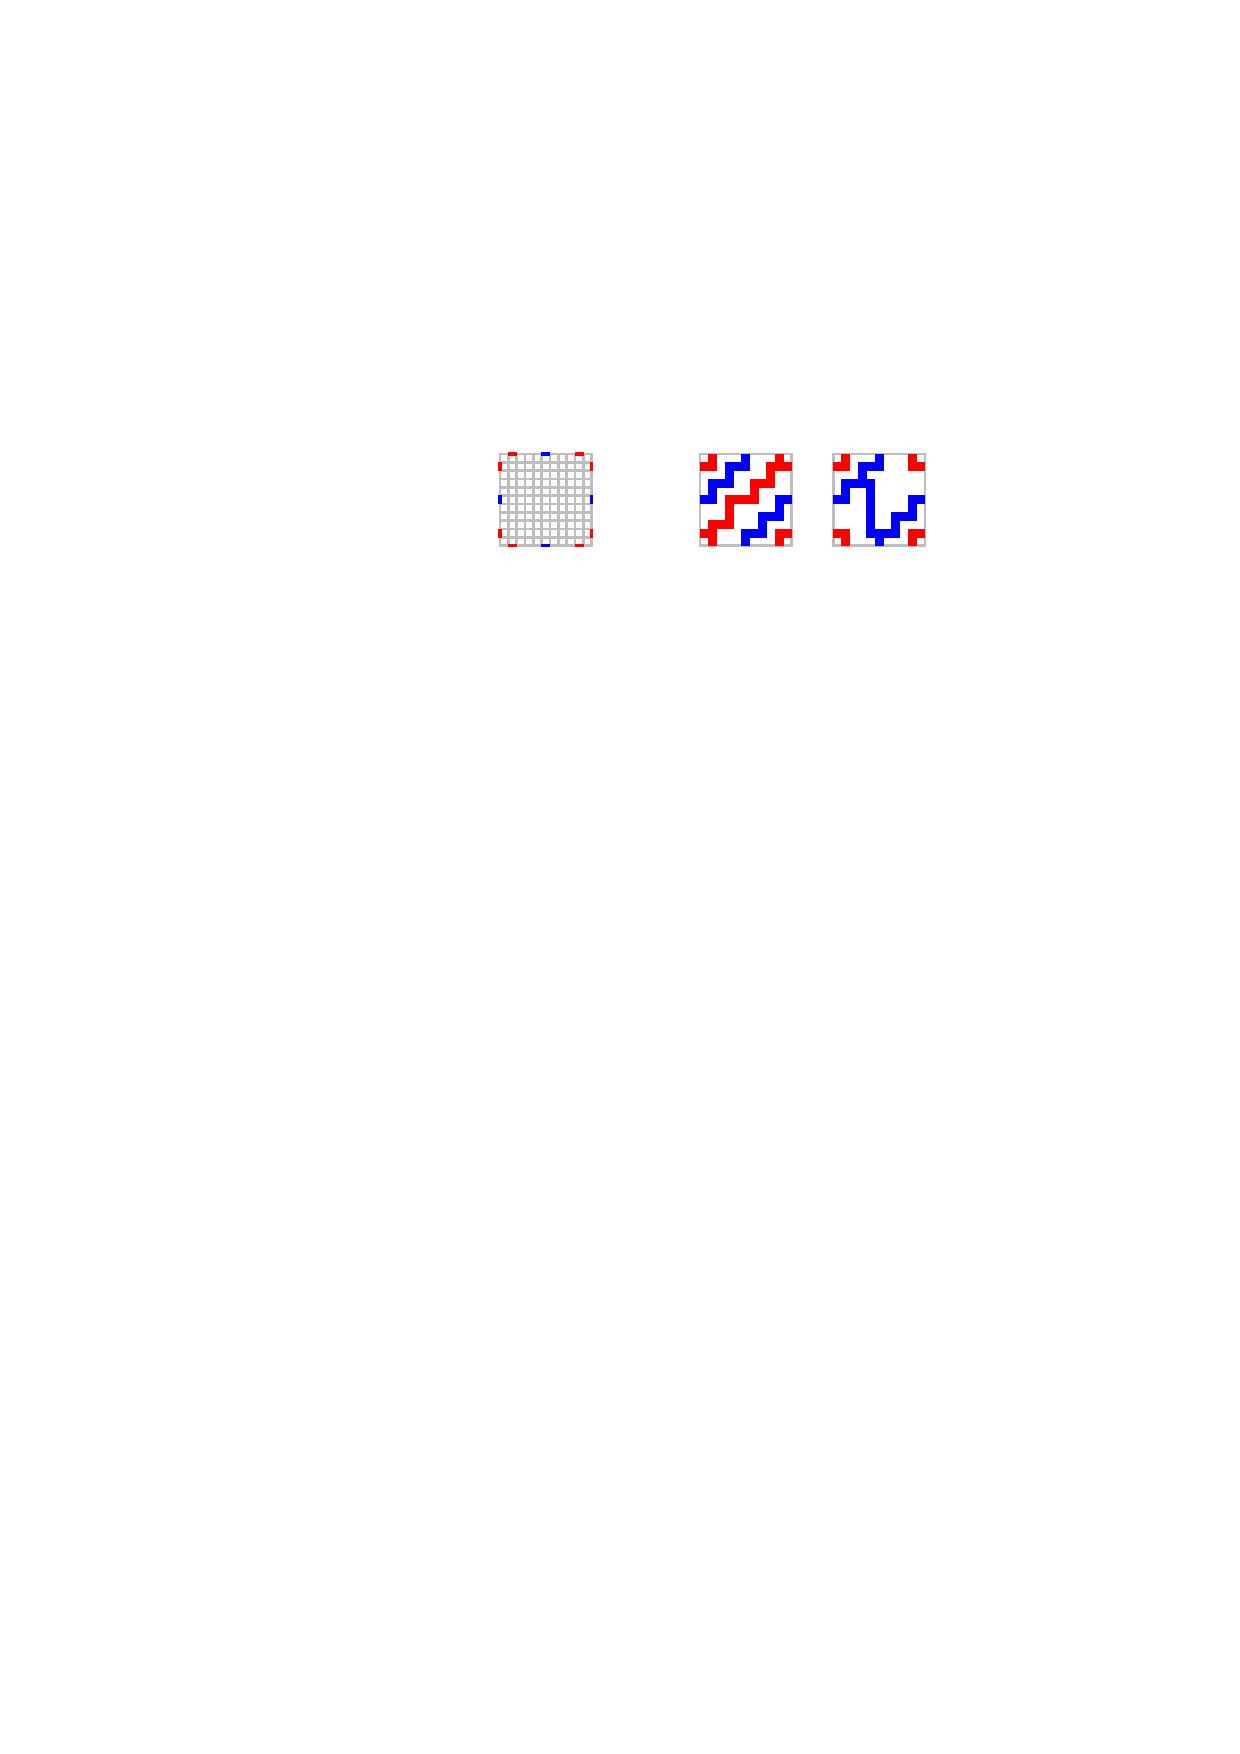
\includegraphics[]{painter-panels.pdf}
\caption{Left, a superpixel showing the locations of the three intervals per side. Right, the two most complex panels represented by superpixels.}
\label{fig:panel}
\end{figure}

In our problem, we have two regions $R_1$ and $R_2$. We create a grid coarsening $\Gamma_{11}$. We record for every superpixel whether it is visited by $R_1$ and/or $R_2$. 
%If $R_i$ covers a superpixel completely, we assign all of its pixels to $P_i$.
Then we forget $R_1$ and $R_2$ altogether and apply the results from \cite{goethem2017painter}. The regions $R_1$ and $R_2$ are the red and the blue region and the superpixels are the panels. Since the recording of colors with panels comes from disjoint simply-connected regions, we know that the 2-colored grid of panels admits a painting, so it admits one as specified in Lemma~\ref{lem:painting}, and we can apply the reductions to simplify the cases.

It remains to show that each of the simplified cases can be represented in an $11\times 11$ superpixel with disjointness of the pieces of $P_1$ and $P_2$. This comes down to checking all cases. The two most complex ones are shown in Figure~\ref{fig:panel}; others are subsets or symmetric variants.

\begin{theorem}
If $\mathcal{R}$ consists of two disjoint, simply-connected regions, it is possible to find a valid assignment such that for each region $R_i \in \mathcal{R}$ with a corresponding region $P_i$, we have $H(R_i, P_i) = \Theta(1)$.
\end{theorem}



\subsection{Three or More Regions}
\label{subsec:three}

\begin{theorem}\label{thm:unbouded}
% The amount of stretch needed to color a screen with three or more polygons is unbounded.
% There are instances of three polygons that can not be ... with
For each $h$ there exists an instance $\mathcal{R}=\{R_1, R_2, R_3\}$, such that there are no $h$-similar grid polygons.
\end{theorem}
\begin{proof}
Assume that there is an $h\in \mathbb{N}$, such that each instance $\mathcal{R}=\{R_1, R_2, R_3\}$ allows $h$-similar grid polygons $\mathcal{P}=\{P_1, P_2, P_3\}$.

Now let $R_1$, $R_2$ and $R_3$ be three regions defined as follows:
\jerome{spiral that loops around $h$ times, see Figure~\ref{fig:arbitrary-spirals}}
The three regions are colored in red green and blue.
Let $\ixi$ be the region containing all points that are within distance $h$ of at least two different regions $R_i$.
%Let $\ell$ be the horizontal line of symmetry of $\ixi$.

\begin{figure}
\centering
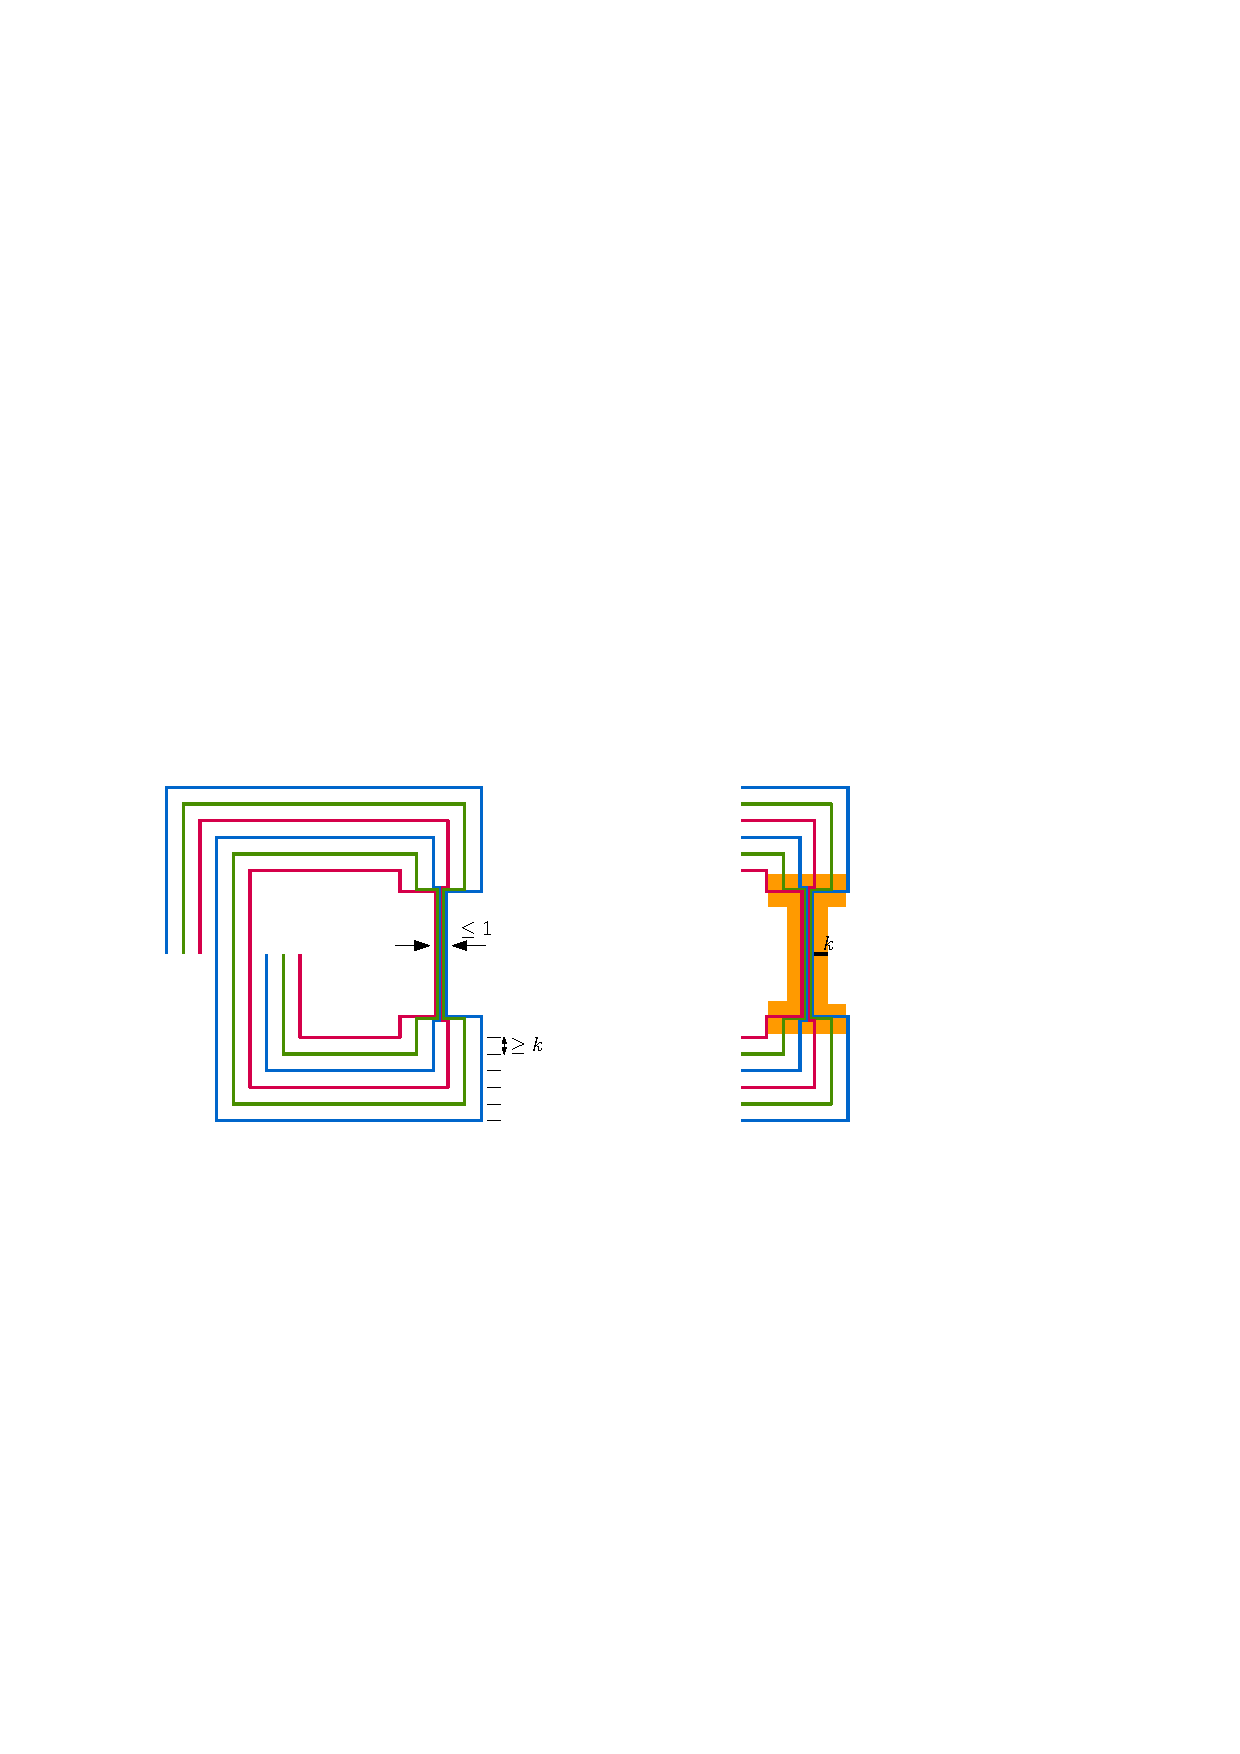
\includegraphics[scale=1]{Figures/arbitrary-lower-by-spirals.pdf}
\caption{The regions for $h=2$. The region $\ixi$ is highlighted in yellow.}
\label{fig:arbitrary-spirals}
\end{figure}

The grid polygons intersect the upper part of the boundary if $\ixi$ in alternating order: red, green, blue, red, \dots

For each $i\in\{1, 2, 3\}$, let $Q_i=P_i\cap \ixi$.
$Q_i$ is a set of grid polygons.
Also let $S_i=P_i\setminus Q_i$.
The set $S_i$ contains $h+1$ grid polygons.
Each separate grid polygon of $Q_i$ connects grid polygons of $S_i$.
Let $Q$ be a grid polygon of $Q_i$. Let $t$ ($b$) be the number of grid polygons of $S_i$ that it touches at the top (bottom) boundary of $\ixi$. We then say that $Q$ has $t-1$ top connections and $b-1$ bottom connections.
If both $t$ and $b$ are non-zero, we say that $Q$ has a middle connection.
In order to connect the polygons in $S_i$ to form the single grid polygon $P_i$, the polygons in $Q_i$ need to make a total of $h$ connections.
So over the three colors a total of $3h$ connections are needed.

We know that in total at most $h-1$ top connections can be made. This stems from he fact that whenever two red polygons of $S_i$ are connected
This is proven as follows:
let $a$ and $b$ be two red grid polygons from $S_1$ that are connected via the top of $\ixi$. Then the green and blue grid polygons of $S_2$ and $S_3$ between $a$ and $b$ can no longer be connected via the top to any green or blue grid polygons of $S_2$ and $S_3$ outside $a$ and $b$.
\jerome{Is this above enough or do we need to elaborate more on this part of the proof?}
The same holds for the bottom connections.

This means that at least $3h- 2(h-1) = h+2$ middle connections exist. However the region $\ixi$ has only width $2h+1$ in the middle, so at most $h$ middle connections can be drawn.
Contradiction.

\end{proof}

% This implies that for three or more polygons the best fitting grid polygons have unbounded..... I do not know how I can phrase this ...

% section arbitrary (end)


\section{Conclusion} % (fold)
\label{sec:conclusion}

In this paper we have shown what Hausdorff distance bounds can be attained when mapping disjoint simply-connected regions to the unit grid. We expressed our bounds in the number of regions and obtained different results depending on the shape and size characteristics of the regions. Our r



Open Questions that can be still researched:
\begin{enumerate}
	\item fat non-convex polygons for interesting fatness definitions. Because for some of them Theorem~\ref{thm:unbouded} holds.
	\item How about two polygons in the general setting? This would create an interesting comparison to either the one polygon or the three polygon cases where one is easy and one is unbounded.
	Solved reading: The Painter’s Problem: Covering a Grid with Colored Connected Polygons
	\item Can we give an algorithm for a stretch depending on the complexity of $A$, i.e., number of vertices, rotation number, \dots?
	\item We can also do a set of point regions and one more arbitrary region without upsetting the $O(\sqrt{m})$ bound. Is this also true for two arbitrary regions with $m$ point regions? Is it also true for convex regions and one or two arbitrary regions? And fat convex?
\end{enumerate}

% section conclusion (end)

\newpage
\appendix

\bibliographystyle{abbrv}

\bibliography{bib}

\end{document}
